\section{Simulated annealing}
\label{sec:simulated-annealing}

Simulated Annealing~\cite{skir83} is a generic probabilistic algorithm
for finding the global optimum of a given function,
$\mathcal{F}: \mathbb{R} \rightarrow \mathbb{R}$, which has a large
search space.  Simulated Annealing in most of the cases is cheaper than
exhaustive enumeration, which is exhaustively listing the entire search
space. Since it is a Monte Carlo method it will always terminate and the
solution need not be the most optimal but in general considered to be a
good approximation of the optimum.

% \subsection{Overview}

% <<<<<<< HEAD
% In general SA is a non-greedy heuristic algorithm which explores the
% search space by moving from a higher temperature to a lower
% temperature. The algorithm always accepts moves to a better solution,
% determined by evaluating an \emph{objective function} and sometimes
% accpets moves to worse states with a probability that changes with
% temperatures. Initially, when the temperature is high, the algorithm is
% more tolerable and accepts moves to worse states with a higher
% probability. As the temperature falls down, this probability decreases
% and the alogrithm is less tolerant towards solutions with a worse value
% for the objective function.

% This is the reason why SA is not a purely greedy algorithm as it accepts
% moves to bad states with some probability which enables it to move out
% of local maximas\/minimas. But the algorithm becomes more greedier as
% the temperature decreases. Figure~\ref{fig:temperature_drop} shows how
% the temperature drops and how this acceptance probability changes with
% this drop in temperature.

% \subsection{From the mapping problem standpoint}

% \begin{algorithm}
%   \DontPrintSemicolon
%   \KwIn{Initial Mapping $\zeta_0$ and Starting Temperature $T_0$}
%   \KwOut{Best Mapping $\zeta_{best}$}
%     $\zeta \leftarrow \zeta_0$\;
%     $C \leftarrow OBJECTIVE\_FUNCTION(\zeta_0)$\;
%     $\zeta_{best} \leftarrow \zeta$\;
%     $C_{best} \leftarrow C$\;
%     \Return $\zeta_{best}$
%   \caption{$Simulated\_Annealing(\zeta_0, T_0)$}
%   \label{algo:SA}
% \end{algorithm}

% Figure~\ref{algo:SA} represents the pseudocode for our algorithm. We
% begin by choosing some initial starting point for our state space
% exploration, which from the mapping problem standpoint is some initial
% mapping of tasks from $V_t$ to PEs $V_r$. We choose our initial mapping
% to be all tasks from $V_t$ mapped onto some random PE $j \in V_r$. This
% is a good idea because we have observed that this puts tightly coupled
% tasks, i.e. tasks that communicate heavily, on the same PE since moving
% them onto different PEs would incur more costs and would thus lead to a
% bad state.
% =======
SA is a heuristic algorithm which explores the search
space by moving from a higher temperature to a lower temperature. The algorithm
always accepts moves to a better solution, determined by evaluating an
\textit{objective function} and sometimes accepts moves to worse states with a
probability that changes with temperature. Initially, when the temperature is
high, the algorithm is more tolerable and accepts moves to worse states with a
higher probability. As the temperature falls down, this probability decreases
and the algorithm is less tolerant towards solutions with a worse value for the
objective function.

This is the reason why SA is not a purely greedy algorithm as it accepts
moves to bad states with some probability which enables it to move out
of local maxima and minima. However, the algorithm becomes greedier as
the temperature decreases. Figure~\ref{fig:7} shows how the temperature
drops for different values of a annealing parameter $q$ which is
described in Sections~\ref{sec:conventional-SA}
and~\ref{sec:our-improved-sa}.

\subsection{Conventional Simulated Annealing : From the mapping problem
  standpoint}
\label{sec:conventional-SA}

\begin{algorithm}[h!]
  \small{
    \caption{$Simulated\_Annealing(\zeta_0, \mathcal{T}_0)$}
    \label{algo:SA}
    % \DontPrintSemicolon
    \KwIn{Initial Mapping $\zeta_0$ and Starting and Final Temperatures
$\mathcal{T}_0$, $\mathcal{T}_f$}
    \KwOut{Best Mapping $\zeta_{best}$}
    $\zeta_{current} \leftarrow \zeta_0$ \;
    $C_{current} \leftarrow OBJECTIVE\_FUNCTION(\zeta_0)$ \;
    $\zeta_{best} \leftarrow \zeta_{current}$\;
    $C_{best} \leftarrow C_{current}$\;
    $R \leftarrow 0$\;
    \For {$i \leftarrow 0\ to\ \infty$}{
      $\mathcal{T}_{current} \leftarrow NEXT\_TEMPERATURE(\mathcal{T_0,i})$\;
      $\zeta_{new} \leftarrow NEXT\_STATE(\zeta_{current}, \mathcal{T})$\;
      $C_{new} \leftarrow OBJECTIVE\_FUNCTION(\zeta_{new})$\;
      $\Delta C \leftarrow C_{new} - C_{current}$\;
      $r \leftarrow RAND()$\;
      $p \leftarrow ACCEPTANCE\_PROBABILITY(\Delta C, \mathcal{T}_{current})$\;
      \If{$\Delta C \textless 0$ or $r \textless p$}{
        \If{$C_{new} \textless C_{best}$}{
          $\zeta_{best} \leftarrow \zeta_{new}$\;
          $C_{best} \leftarrow C_{new}$\;
          $\zeta_{current} \leftarrow \zeta_{new}$\;
          $C_{current} \leftarrow C_{new}$\;
          $R \leftarrow 0$\;
        }
      }
      \Else{
        \If{$\mathcal{T}_{current} \leq \mathcal{T}_f$}{
          $R \leftarrow R+1$\;
          \If{$R \geq R_{max}$}{break}
        }
      }
    }
    \Return $\zeta_{best}$
  }
\end{algorithm}

Algorithm~\ref{algo:SA} represents the pseudo-code for the novel
algorithm presented by ~\cite{hors06} which maps applications onto
Multiprocessor SoCs.  The \textit{OBJECTIVE\_FUNCTION} evaluates
execution time of a specific mapping by calling the
scheduler. $\zeta_0,\ \zeta_{current}$ and $\mathcal{T}_0,\
\mathcal{T}_{current}$ are the initial and current mapping and
temperatures, respectively. The \textit{NEXT\_STATE} function moves a
random task to a random PE different than the original
PE. \textit{NEXT\_TEMPERATURE} is chosen so that the annealing schedule
is proportional to the number of tasks and resources and is given by,

\begin{equation}
\label{eq:3}
\textit{NEXT\_TEMPERATURE}(\mathcal{T}_0, i) = \mathcal{T}_0*q^{\lfloor
\frac{i}{L} \rfloor}
\end{equation}
\noindent
where q is the proportion of temperature preserved in each temperature
level. % In their paper, q was set as $0.95$ and
L is the number of iterations in one temperature level. Multiple
iterations are achieved at a single temperature level by using the
\texttt{floor} function, since $\lfloor \frac{i}{L} \rfloor$ moves to a
new value only at every integral multiple of $L$.

\begin{equation}
L = |V_t|*(|V_r| - 1)
\end{equation}

The \textit{ACCEPTANCE\_PROBABILITY} function is modified from its
traditional form: $\frac{1}{1+exp(\frac{\Delta C}{\mathcal{T}})}$ to
adapt automatically to different cost function value ranges and graphs
with different task execution times. This is done by normalizing the
change in cost, $\Delta C$,

\begin{equation}
  \begin{array}{c}
    ACCEPTANCE\_PROBABILITY(\Delta C, \mathcal{T}) \\ 
    = \frac{1}{1+exp(\frac{\Delta C}{0.5C_0\mathcal{T}})}
  \end{array}
\end{equation}

The initial temperature $\mathcal{T}_0$ of the annealing schedule is
selected as:

\begin{equation}
\mathcal{T}_0 = \frac{t_{max}}{t_{minsum}}
\end{equation}
\noindent
where $t_{max}$ is the maximum execution time for any task $i \in V_t$
on any PE $j \in V_r$ and $t_{minsum}$ is the sum of execution time of
all tasks in $V_t$ on the fastest PE $j_{fastest} \in V_r$.

The final temperature of the annealing schedule is selected as:

\begin{equation}
\mathcal{T}_f = \frac{t_{min}}{t_{maxsum}}
\end{equation}
\noindent
where $t_{min}$ is the minimum execution time for any task $i \in V_t$
on any PE $j \in V_r$ and $t_{maxsum}$ is the sum of execution time of
all tasks in $V_t$ on the slowest PE $j_{slowest} \in
V_r$. % In both the
% cases, $k$ is a constant and $k=1$ is suitable for all our experiments.

\subsection{Our Improved SA Approach}
\label{sec:our-improved-sa}

We made novel changes to the aforementioned algorithm and associated
heuristics as prescribed by Orsilla et al~\cite{hors06}. The reasons
behind these changes are two fold.

\begin{itemize}
\item We need to suit map the task graph onto a heterogeneous execution
  architecture.

\item We need to improve the annealing schedule in order to obtain
  better application latencies.

\item We need to improve the run-time of the SA algorithm to scale to
  large processor architectures.
\end{itemize}

Our list of changes to the standard SA heuristic are as follows:

\begin{itemize}

\item We begin by choosing some initial starting point for our state space exploration, which from
the mapping problem standpoint is some initial mapping of tasks from $V_t$ to
PEs $\in V_r$, to be all tasks from $V_t$ mapped onto
some random PE $j \in V_r$. This is a good idea because we have observed that
this puts tightly coupled tasks, i.e. tasks that communicate heavily, on the
same PE and moving them onto different PEs would incur more communication
costs and would thus lead to increased application latency.

\item The \textit{OBJECTIVE\_FUNCTION} evaluates the latency of execution of
the mapping $\zeta$ on $V_r$ as described earlier in
Section~\ref{sec:relat-notat-form}. 

\item The \mbox{\textit{NEXT\_STATE ($\zeta_{current}$, $T_{current}$)}}
  function describes how we are going to move to a new state. This is
  one of the \underline{most important contribution} of this paper. We
  make this movement to a new state, a function of the current state and
  current temperature $\zeta_{current}$,
  $\mathcal{T}_{current}$. Consider a given mapping $\zeta_\mathcal{M}$
  which maps $V_t$ to $V_r$. When the temperature is high, we allow a
  lot of the elements in this mapping of the form $r_i \leftarrow t_k$
  to change to mappings of the form $r_j \leftarrow t_k$. This means we
  allow a lot of tasks to migrate to different PEs when the temperature
  is high. As the temperature decreases, we restrict the motion of these
  tasks, meaning we allow only fewer tasks to migrate to different PEs
  and enforce a condition on the rest of the tasks to stay at the PE
  they are currently in. It should also be kept in mind that during
  every iteration, the tasks that are allowed to move are selected at
  random while the number of tasks that have to be moved will be guided
  by the temperature. The reason for doing this is two fold,
\begin{itemize}
\item We want to explore different corners of the search space when the
  temperature is high.
\item As the temperature drops, we want to reduce our search space to
  the current best solutions neighborhood.
\end{itemize}
This can be thought of as doing a global state space exploration at the
beginning stages of the optimization, i.e. when temperature is high, as
we want to get a sense of which neighbourhood gives a good result. Once
we find a good neighbourhood we start to reduce our radius of search by
allowing only limited number of tasks to move to different PEs. This
results in a localized search when the temperature drops. We found this
to be quite effective in terms of finding effective mappings as our
results from Section~\ref{sec:results} shows.

\item The \textit{NEXT\_TEMPERATURE} function, which is defined in
  Equation~(\ref{eq:3}), is also changed to prevent multiple mapping
  iterations in one temperature level. We want to avoid this as we do
  not want to spend a majority of the annealing schedule searching for
  global optimums.

\begin{equation}
  \textit{NEXT\_TEMPERATURE}(\mathcal{T}_0, i) =
  \mathcal{T}_0*q^{\frac{i}{L}}
\end{equation}

\begin{figure}[h!]
  \centering
  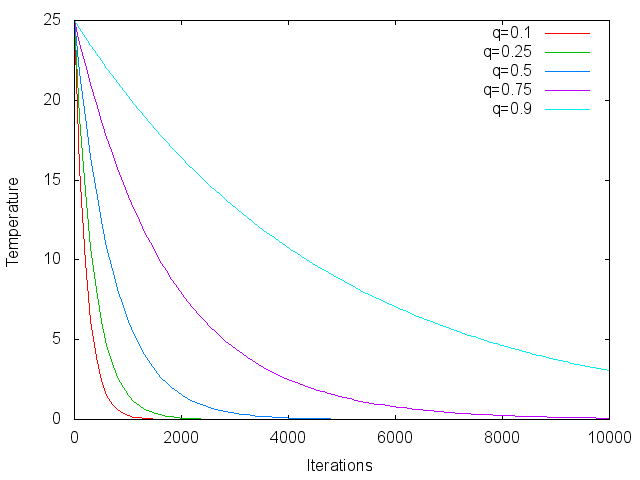
\includegraphics[scale=0.35]{./figures/temperature-drop}
  \caption{Temperature variations in standard SA with varying $q$}
  \label{fig:7}
\end{figure}
Figure~\ref{fig:7} shows how the temperature varies with iterations. It
clearly shows how the temperature drops quicker for smaller values of
$q$ and slower for larger values. Even though we removed the concept of
multiple number of mapping iterations per temperature level from the
previous algorithm, we retained the $q$ parameter as we wanted to
control how quickly or slowly the temperature must drop.

\item We use the value for the initial and final temperature for the
  annealing schedule from the paper written by Orsilla et
  al.~\cite{hors06}. Since the objective of this article is to map
  heterogeneous applications onto heterogeneous architectures, these
  heuristics have to be changed as well. We calculate the fastest and
  slowest processors by multiplying each processor's capabilities
  ($W^r_0(i) * W^r_1(i)$) and sorting them.

% \item The rest of the parameters remain the same as~\cite{hors06} and are subject to future work
% for changes if necessary.

\end{itemize} 

%%% Local Variables: 
%%% mode: latex
%%% TeX-master: "bare_conf"
%%% End: 
